\chapter{Analóg áramkörök digitális modellezése}

\section{Lineáris áramkörök modellezése}

A lineáris áramkörök modellezésének a leggyakoribb módszereit említem meg~\cite{transformations}~\cite{eulers}.

Egy lineáris, idő-invariáns rendszert pontosan jellemez az átviteli függvénye, aminek a definíciója  a kimenet 
Laplace-transzformáltjának és a bemenet Laplace-transzformáltjának hányadosa.
\begin{equation}
    H(s)=\frac{Y(s)}{U(s)}
\end{equation}
Ennek a videlkedésnek a megvalósítása a cél diszkrét időben.

Lehetséges az a megközelítés is, hogy az állapotváltozós leírás alapján kifejezett rendszert szimulálunk. Ekkor minden belső változó is számolható lenne, de a leggyakoribb esetekben erre nincs szükség, és csak a rendszer kimenete lényeges. Az állapotváltozós leírás alapján való szimuláció több egyenlet megoldását igényelné, így a minél kisebb számítási igény céljából lineáris hálózat esetén kerülendő.

Az összes alább mutatott diszkretizálási módszerek alkalmazásakor behelyettesítés után az átviteli függvény az alábbi alakot veszi fel:
\begin{equation}
    \frac{Y(z)}{U(z)}=\frac{\sum_{i=0}^{N}b_i z^{-i}}{1+\sum_{j=1}^{M}a_j z^{-j}}
\end{equation}
Ezt az egyenletet átrendezve:
\begin{equation}
    Y(z)(1+\sum_{j=1}^{M}a_j z^{-j})=U(z)\sum_{i=0}^{N}b_i z^{-i}
\end{equation}
\begin{equation}
    Y(z)+\sum_{j=1}^{M}a_j Y(z)z^{-j}=\sum_{i=0}^{N}b_i U(z)z^{-i}
\end{equation}
\begin{equation}
    Y(z)=\sum_{j=1}^{M}-a_j Y(z)z^{-j}+\sum_{i=0}^{N}b_i U(z)z^{-i}
\end{equation}
Inverz z-transzormálva megkapjuk a rendszeregyenletet:
\begin{equation}
    y[n]=\sum_{j=1}^{M}-a_j y[n-j]+\sum_{i=0}^{N}b_i u[n-i]
\end{equation}

A szimuláció során ezt az egyenletet kell leprogramozni, ahol az $y$ változónak (válasz) az utolsó $M$ értékét, az $u$ változónak (gerjesztés) pedig az utolsó $N$ értékét kell eltárolnunk a válasz következő értékének számolásához. A bufferelést érdemes cirkuláris bufferrel megvalósítani a számítási igény csökkentésének érdekében. 

\subsection{Előrelépő Euler-módszer}\label{fwEulerSection}

Az előrelépő (explicit) Euler-módszer a deriváltat a következő és az aktuális állapotváltozóból fejezi ki, a többi tagnak
az ezelőtti állapotát használja.
\begin{equation}
    \mathbf{\dot{w}}=\frac{\mathbf{w}[n+1]-\mathbf{w}[n]}{\Delta{}t}
\label{fwEuler}
\end{equation}
\begin{equation}
    \mathbf{\dot{w}}=\frac{\mathbf{w}[n+1]-\mathbf{w}[n]}{\Delta{}t}=\mathbf{A}\mathbf{w}[n]+\mathbf{Bu}[n]
\end{equation}
Az $s$-re kifejezve~\ref{fwEuler} alapján:
\begin{equation}
    s=\frac{z-1}{T}=\frac{1-z^{-1}}{Tz^{-1}}
\label{fwEulers}
\end{equation}

Az előrelépő Euler-módszer nem mindig fog stabil folytonos idejű rendszerből stabil diszkrét idejű rendszert 
eredményezni, ami~\ref{fwEulers}-ből egyértelműen kifejezhető~\cite{transformations}. A stabilitás függeni fog a mintavételi frekvenciától, és ha az nem elég nagy, akkor instabil lesz a diszkretizált rendszer.
\begin{equation}
    z=sT+1
\end{equation}

\begin{figure}[!h]
    \centering
    \begin{subfigure}{0.47\textwidth}
        \centering
        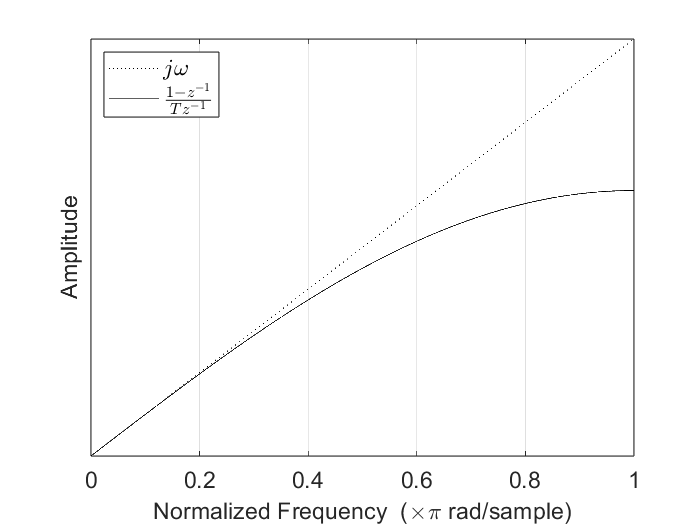
\includegraphics[scale=0.38]{figures/fwEulerA.png}
        \caption{}
    \end{subfigure}
    \hfill
    \begin{subfigure}{0.47\textwidth}
        \centering
        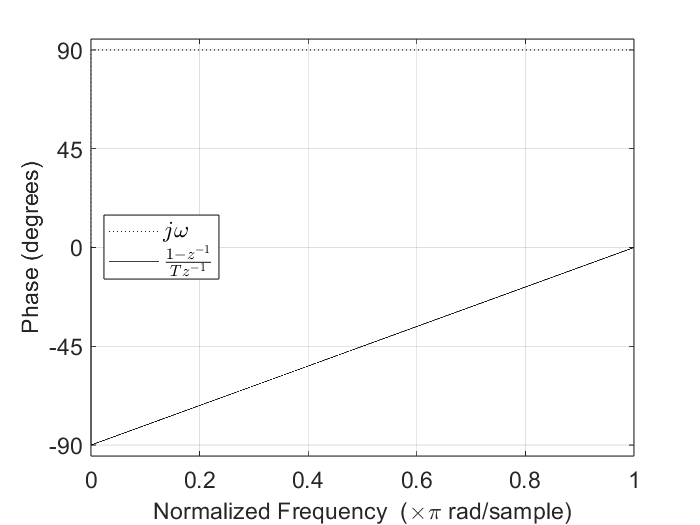
\includegraphics[scale=0.38]{figures/fwEulerP.png}
        \caption{}
    \end{subfigure}
    \caption{Az előrelépő Euler-módszer frekvenciatorzítása}
\end{figure}

\begin{figure}[H]
    \centering
    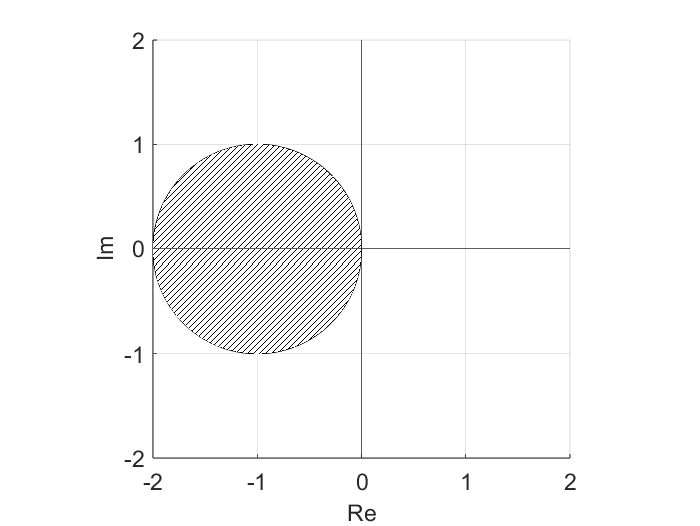
\includegraphics[scale=0.5]{figures/fwEulerS.png}
    \caption{Az előrelépő Euler-módszer alkalmazásával létrehozott diszkrét rendszer stabilitásának feltétele: az $sT$ szorzatnak az ábrán jelölt tartományom belül kell lennie}
\end{figure}

\subsection{Hátralépő Euler-módszer}\label{bwEulerSection}

A hátralépő (implicit) Euler-módszer a deriváltat az aktuális és az ezelőtti állapotváltozóból fejezi ki, a többi tagnak
az aktuális állapotát használja.
\begin{equation}
    \mathbf{\dot{w}}=\frac{\mathbf{w}[n]-\mathbf{w}[n-1]}{\Delta{}t}
\label{bwEuler}
\end{equation}
\begin{equation}
    \mathbf{\dot{w}}=\frac{\mathbf{w}[n]-\mathbf{w}[n-1]}{\Delta{}t}=\mathbf{A}\mathbf{w}[n]+\mathbf{Bu}[n]
\end{equation}
Az $s$-re kifejezve~\ref{bwEuler} alapján:
\begin{equation}
    s=\frac{1-z^{-1}}{T}=\frac{z-1}{Tz}
\label{bwEulers}
\end{equation}
A hátralépő Euler-módszerrel modellezett folytonos idejű rendszer mindig stabil diszkrét idejű rendszerhez vezet, 
ami~\ref{bwEulers} alapján belátható~\cite{transformations}.  
\begin{equation}
    z=\frac{1}{1-sT}
\end{equation}

\begin{figure}[!h]
    \centering
    \begin{subfigure}{0.47\textwidth}
        \centering
        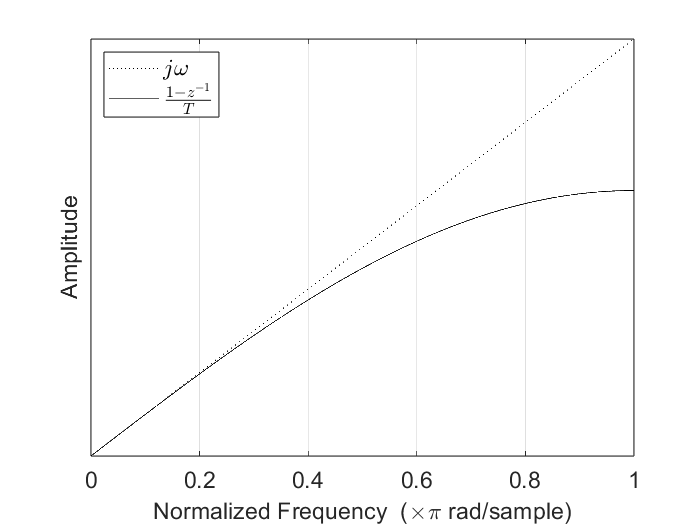
\includegraphics[scale=0.38]{figures/bwEulerA.png}
        \caption{}
    \end{subfigure}
    \hfill
    \begin{subfigure}{0.47\textwidth}
        \centering
        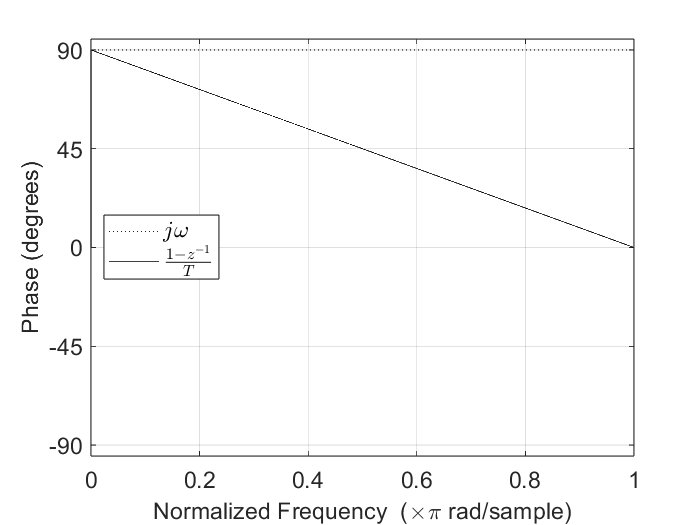
\includegraphics[scale=0.38]{figures/bwEulerP.png}
        \caption{}
    \end{subfigure}
    \caption{A hátralépő Euler-módszer frekvenciatorzítása}
\end{figure}

\begin{figure}[H]
    \centering
    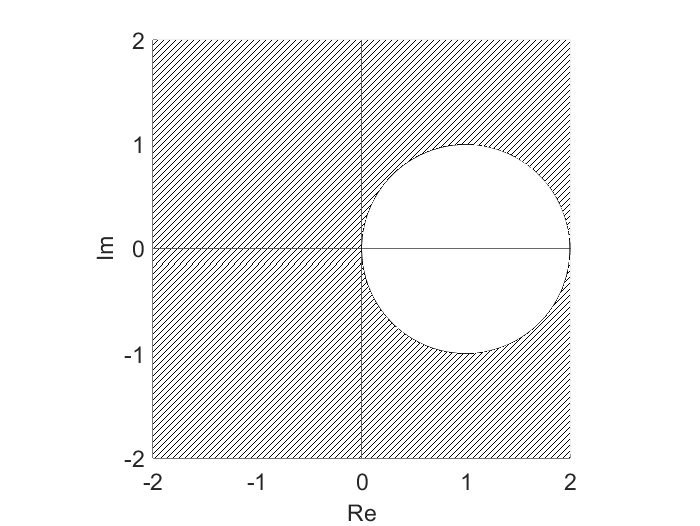
\includegraphics[scale=0.5]{figures/bwEulerS.png}
    \caption{A hátralépő Euler-módszer alkalmazásával létrehozott diszkrét rendszer stabilitásának feltétele: az $sT$ szorzatnak az ábrán jelölt tartományom belül kell lennie}
\end{figure}

\subsection{Bilineáris transzformáció}

Egyik leggyakrabban használt módszer a bilineáris transzformáció, amely az s-síkból a z-síkba transzformál a trapézszabály, azaz 
az előre- és a hátralépő Euler-módszer átlaga szerint.
\begin{equation}
    s=\frac{2}{T}\frac{z-1}{z+1}=\frac{2}{T}\frac{1-z^{-1}}{1+z^{-1}}
    \label{bilin}
\end{equation}
A transzformáció után a rendszer stabilitása megmarad, amit~\ref{bilin}-ből könnyen ki lehet fejezni~\cite{transformations}.

\begin{equation}
    z=-\frac{4}{sT-2}-1
\end{equation}

\begin{figure}[!h]
    \centering
    \begin{subfigure}{0.47\textwidth}
        \centering
        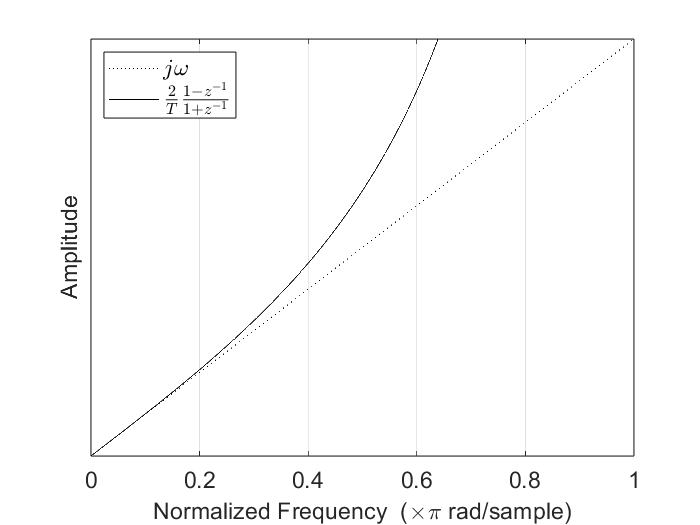
\includegraphics[scale=0.38]{figures/bilinearA.png}
        \caption{}
    \end{subfigure}
    \hfill
    \begin{subfigure}{0.47\textwidth}
        \centering
        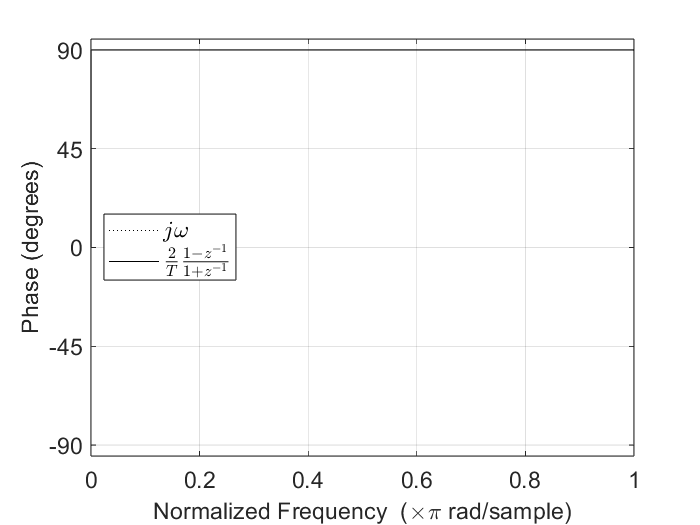
\includegraphics[scale=0.38]{figures/bilinearP.png}
        \caption{}
    \end{subfigure}
    \caption{A bilineáris transzformáció frekvenciatorzítása}
\end{figure}

\begin{figure}[H]
    \centering
    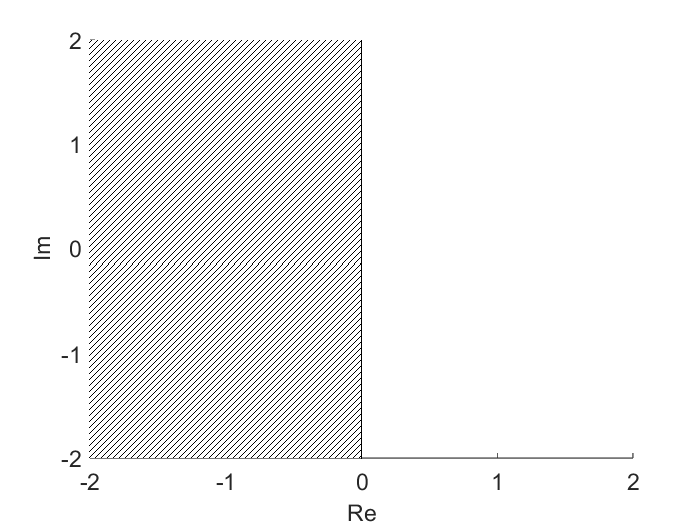
\includegraphics[scale=0.5]{figures/bilinearS.png}
    \caption{A bilineáris transzformáció alkalmazásával létrehozott diszkrét rendszer stabilitásának feltétele: az $sT$ szorzatnak az ábrán jelölt tartományom belül kell lennie}
\end{figure}
Az ábrák alapján látszólag a hátralépő Euler-módszer szerinti diszkretizálás célszerűbb, viszont ez nem így van. A bilineáris transzformációval diszkretizált megoldás pontosabb, hiszen a derivált pontosabban van közelítve (a Taylor-sorának első elemével). A végeredményben így kisebb a hiba a kimenetben, mint a hátralépő Euler-módszer szerinti diszkretizálás esetén.
\subsection{Impulzus invariáns transzformáció}

Az impulzus invariáns transzformációhoz ugyanúgy szükség van a transzformálni kívánt rendszer átviteli függvényére.
\begin{equation}
    H(s)=\frac{B(s)}{A(s)}\triangleq\frac{b_0s^{N-1}+b_1s^{N-2}+\cdots+b_{N-2}s+b_{N-1}}{s^N+a_1s^{N-1}+\cdots+a_{N-1}s+b_{N}}
\end{equation}
Az átviteli függvényt részlettörtekre bontva, inverz Laplace-transzformálva, majd mintavételezve:
\begin{equation}
    H(s)=\sum_{i=1}^{N}\frac{K_i}{s-s_i}
\end{equation}
\begin{equation}
    h(t)=\sum_{i=1}^{N}K_i e^{s_i t}
\end{equation}
\begin{equation}
    h[n]=\sum_{i=1}^{N}K_i e^{s_i nT}
\end{equation}
Ezt z-transzformálva kapjuk meg az impulzus-invariáns transzformáció segítségével megtervezett digitális 
szűrőt.
\begin{equation}
    H(z)=\sum_{i=1}^{N}\frac{K_i}{1-e^{s_i T}z^{-1}}
    \label{impinv}
\end{equation}


A transzformáció után a rendszer stabilitása megmarad, hiszen a transzformáció során $s$ és $z$ között a pontos összefüggést használjuk, és nem közelítünk~\cite{transformations}. 
\begin{equation}
    z_i\triangleq e^{s_i T}
\end{equation} 
Ennek köszönhetően frekvenciatorzítás sem lép fel a transzformáció után.




\section{Nemlineáris elemek}
Ha a rendszerbe memória nélküli nemlinearitás kerül, akkor az átviteli függvény nem értelmezett.

Az állapotváltzós leírás egy differenciálegyenlet rendszer, ami egy hálózatot pontosan meghatároz. Mivel az átviteli függvény nem értelmezett a nemlinearitás miatt, így az állapotváltozós leírás segítségével kell modellezni a hálózatot. Ekkor az állapotváltozós leírásban 
meg fog jelenni a nemlineáris függvény.
\begin{equation}
    \mathbf{\dot{w}}(t)=\mathbf{A}\mathbf{w}(t)+\mathbf{Bu}(t)+\mathbf{Cf}(\mathbf{w}(t),\mathbf{u}(t))
\end{equation}

Leggyakrabban a megoldáshoz az Euler-módszerek és a Runge-Kutta módszerek használatosak~\cite{eulers}~\cite{rungekutta}~\cite{rkk}.

\subsection{Előrelépő Euler-módszer}
Az előrelépő Euler-módszer használatánál az egyenletrendszer gyakran egyszerűen megoldható lesz, átrendezés után az előző 
állapotokat behelyettesítve kapható meg a következő állapot.

Diszkretizáláshoz a (\ref{bwEulers}) egyenletet használandó, ezt behelyettesítve, és rendezve:
\begin{equation}
    \mathbf{w}[n+1]=\mathbf{A'}\mathbf{w}[n]+\mathbf{B'u}[n]+\mathbf{C'f}(\mathbf{w}[n], \mathbf{u}[n])
\end{equation}
Ezt átrendezve:
\begin{equation}
    \mathbf{w}[n]=\mathbf{A'}\mathbf{w}[n-1]+\mathbf{B'u}[n-1]+\mathbf{C'f}(\mathbf{w}[n-1],\mathbf{u}[n-1])
\end{equation}
Az átalakítások után sok esetben csak a korábbi értékeinket be kell helyettesítenünk az explicit egyenletbe a következő minta számolásához.

Ahogy a~\ref{fwEulerSection} részben látható, lehetséges, hogy a diszkretizált rendszer instabil lesz. Ez a mintavételi frekvenciától függ, és gyakran ez nagyon nagy frekvencia esetén lesz csak stabil a rendszer. Ez a feltétel legtöbbször nem teljesíthető valós idejű szimuláció esetén, így ritkán használatos.

\subsection{Hátralépő Euler-módszer}
A hátrelépő Euler-módszer használatával új problémák merülnek fel, viszont a stabilitási kérdés megoldódik. 
Az állapotváltozós leírás transzformálása és rendezése egy implicit egyenletrendszerhez vezet.
\begin{equation}
    \mathbf{w}[n]=\mathbf{A'}\mathbf{w}[n-1]+\mathbf{B'u}[n]+\mathbf{C'f}(\mathbf{w}[n],\mathbf{u}[n])
\end{equation}
Látható, hogy az egyenletrendszer bal és jobb oldalán is (jobb oldalon a függvény argumentumaként) megtalálható az $\mathbf{w}[n]$ állapotváltozó. Az implicit egyenlet valamely zérushely-kereső algoritmussal megoldandó 
(intervallumfelezés, Newton-módszer, szelőmódszer stb.~\cite{bookNewton}). A nehézségeket pedig az ellensúlyozza, hogy az implicit egyenlet megoldásának árán stabil folytonos idejű rendszerből stabil diszkrét idejű rendszer lesz.

\subsection{Negyedfokú Runge-Kutta módszer}
A Runge-Kutta módszereket gyakran szokták használni nemlineáris rendszerek offline szimulációjánál. Alapötletük hasonló, mint az Euler-módszereknek, viszont itt több pontból közelítik a deriváltat. Így ha a az eredeti rendszernek a nagyon pontos modellezése a cél, akkor jobb eredményt biztosítanak, mint az Euler-módszerek. Viszont nagyobb a számításigényük, és nem alkalmazhatóak valós időben, hiszen a számításhoz gerjesztést szükséges olyan pontokban is ismerni, ami általában egy valós idejű alkalmaás esetén nem lehetséges. Leggyakrabban használt verziója a negyedfokú Runge-Kutta módszer (RK4)~\cite{rkk}~\cite{rungekutta}.

A negyedfokú Runge-Kutta (RK4) módszerre a matematikusok a leghatékonyabb numerikus közönséges differenciálegyenlet megoldó módszerként hivatkoznak~\cite{rk4}, mert a magasabb fokú változatok a pontosságot csak kis mértékben tudják növelni a hozzáadott nagy számítási igény mellett. A módszer alapfeltétele, hogy ismert a nemlineáris differenciálegyenlet, és a kezdeti értékek adottak:
\begin{equation}
    \begin{cases}
        \mathbf{\dot{w}}=f(\mathbf{w}(t), \mathbf{u}(t))\\
        \mathbf{w}(t_0)=\mathbf{w_0} 
    \end{cases}
\end{equation}
Ekkor legyen $h=T$, és felírható:
\begin{equation}
    \begin{cases}
        w[n+1]=w[n]+u[n]+\frac{h}{6}(K_1+2K_2+2K_3+K_4)\\
        K_1=f(w[n], u(nT))\\
        K_2=f(w[n]+h\frac{K_1}{2}, u(nT+\frac{h}{2}))\\
        K_3=f(w[n]+h\frac{K_2}{2}, u(nT+\frac{h}{2}))\\
        K_4=f(w[n]+hK_3, u(nT+h))
    \end{cases}
\end{equation}
Ebben az egyenletrendszerben:
\begin{itemize}
    \item $K_1$ a függvény meredeksége az intervallum kezdetén $y$ alapján számítva
    \item $K_2$ a függvény meredeksége a intervallum közepén $y$ és $K_1$ alapján számolva 
    \item $K_3$ a függvény meredeksége a intervallum közepén $y$ és $K_2$ alapján számolva
    \item $K_4$ a függvény meredeksége a intervallum végén $y$ és $K_3$ alapján számolva
\end{itemize}
Mint látható, $K_2$ és $K_3$ számolásához szükség lenne a gerjesztés két mintavételezési pont közötti értékére, így valós időben nem, vagy csak nehezen alkalmazható.